\section{Softwareimplementierung}
\paragraph{}
\subsection{Vergleich Monolithische Single Application und Service Oriented Architecture}
\subsubsection{Monolithische Single Application}
\paragraph{}
Wie es häufig in der Entwicklung der Fall ist, stehen auch hier für die Implementierung
der Software auf dem RPi verschiedene Plattformen, Frameworks und
Programmiersprachen zu Verfügung. Bei der Programmiersprache viel die Wahl recht
schnell auf Python, da es einem im Vergleich zu C/C++, aber auch Java viel Overhead
abnimmt, in der allgemeinen Komplexität geringer ist und vielerorts (wie auch in ROS,
siehe unten) nativ unterstützt wird.
\paragraph{}
Bei der Softwarearchitektur wurde sich zunächst an einer normalen objektorientierten Struktur bedient: Es gibt eine main-Datei, welche vergleichsweise
klein ist und nur die grobe Struktur bzw. den Gesamtablauf darstellt. Diese ruft dann weitere Softwaremodule auf, die die Unteraufgaben, wie beispielsweise das Empfangen und Verarbeiten von Bilddaten, implementiert. Ein Problem, das hier recht schnell auftritt ist, dass theoretisch zwei Prozesse gleichzeitig ablaufen müssen. Wenn ein Motormodul beispielsweise gerade darauf wartet, dass die Sollposition erreicht wurde, müsste in einem Programmierstrang, in dem ein Befehl nach dem anderen ausgeführt wird, das Kameramodul mit der Verarbeitung des Bildes auf das Motormodul warten, obwohl das Motormodul gerade gar nichts tut, außer auf den
Motor in der echten Welt zu warten, bis er die gewünschte Position hat. Da das Kameramodul aber an das Motormodul eventuell kommunizieren muss, dass das
Paket gar nicht mehr an der richtigen Stelle ist, weil der Quadrokopter aufgrund äußerer Umstände nicht ganz stillsteht, müssen beide Module gleichzeitig arbeiten und
miteinander kommunizieren können. 
\paragraph{}
In der traditionellen Softwareentwicklung gibt es dafür sogenannte Threads. Diese sind separate Ausführungsstränge, die quasi gleichzeitig ausgeführt werden und sich dann beispielsweise ein Datenobjekt im Speicher teilen und über dieses miteinander kommunizieren können. Das entspricht dann einer Dreischicht-Architektur.
\begin{figure}[h]
	\centering
	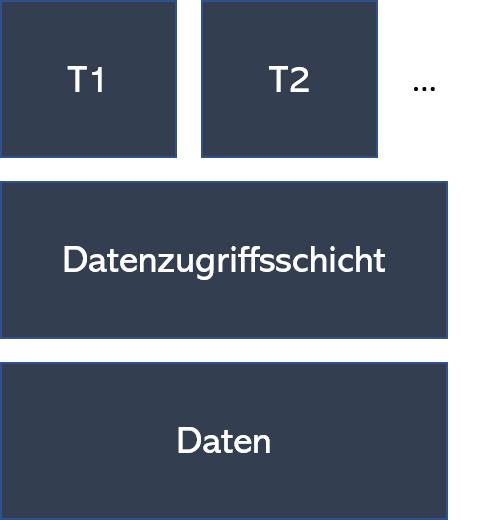
\includegraphics[scale=0.5]{"Grafiken/dreischichtarchitektur.png"}
	\caption{Dreischichtarchitektur}
	\label{fig:meine-grafik}
\end{figure}
Wichtig bei dieser Art der Architektur ist, dass jede Schicht nur auf die nächst untere zugreifen darf, um einen reibungslosen Ablauf garantieren zu können. In diesem Fall greifen nun die Threads $T_1$, $T_2$ ... $T_n$ nicht direkt auf den Speicher zu, sondern müssen den Weg über die Datenzugriffsschicht gehen. Diese stellt unter anderem mittels Semaphoren sicher, dass immer nur ein Thread auf die entsprechende Ressource zugreifen kann. Damit wird verhindert, dass beispielsweise $T_1$ schreiben und $T_2$ gleichzeitig lesen möchte. Dies würde zu einem Speicherkonflikt führen und das Programm wird abstürzen. \cite{riedel2019itarch}

\subsubsection{Service Oriented Architecture}
\paragraph{}
Bis zu einem gewissen Grad war es möglich die geforderten Funktionalitäten mit Multithreading zu implementieren. Allerdings wurde es im Laufe der Entwicklung immer komplizierter, da Bilddaten beispielsweise von zwei Ressourcen abhängen, die nicht immer verfügbar sind: zum einen der Speicherplatz im Datenobjekt, das andere Threads lesen und damit belegen wollen und zum anderen von der Kamera selbst, die natürlich auch nicht willkürlich Bilddaten liefert. Das zu synchronisieren ist zwar theoretisch möglich, praktisch aber mit einer Menge schwer wartbarem Code verbunden, der das Problem unnötig kompliziert löst.
\paragraph{Robot Operating System}
Deshalb basiert die endgültige Software auf ROS, das genau diese Probleme adressiert. ROS steht dabei für Robot Operating System und ist ein Framework, das auf dem Publisher-Subscriber-Modell basiert. Die Idee ist dabei, dass es verschiedene Themen (Topics) gibt, in die verschiedene dezentrale Skripte, die gleichzeitig laufen, Informationen zu einzelnen Themen veröffentlichen oder abonnieren können. So gibt es beispielsweise ein Kameraskript, das das Bild und die erkannte Position des Pakets veröffentlicht und ein Motorskript abonniert die Paketposition und kann daraus dann weitere Schlüsse ziehen. Ein anderes Skript könnte dann auf einem anderen Rechner (z.B. Laptop) im gleichen (WLAN-) Netzwerk das Kamerabild abbonnieren und mit sehr wenig Programmieraufwand anzeigen. Das elegante dabei ist, dass sämtliche vorher beschriebene Multithreading-Probleme dabei vom sogenannten ROS-Core, der zentrale Schaltstelle des ROS, übernommen werden und damit die einzelnen (selbstgeschriebenen) Skripte sehr entschlackt werden. Das macht es deutlich einfacher diese zu debuggen. ROS ist zudem sehr gut dokumentiert und für viele Probleme gibt es bereits vorgefertigte Skripte, die Dank des einfachen P/S-Modells auch einfach anzubinden sind.

\paragraph{ROS als Beispiel einer Service Oriented Architecture (SOA) / Microservices}
Die Architektur hinter ROS ist dabei keine neue Erfindungen, sondern basiert im Gegensatz zum Ansatz der Schichtenarchitektur auf dem Prinzip der serviceorientierten Architektur (SOA). 
\begin{figure}[h]
	\centering
	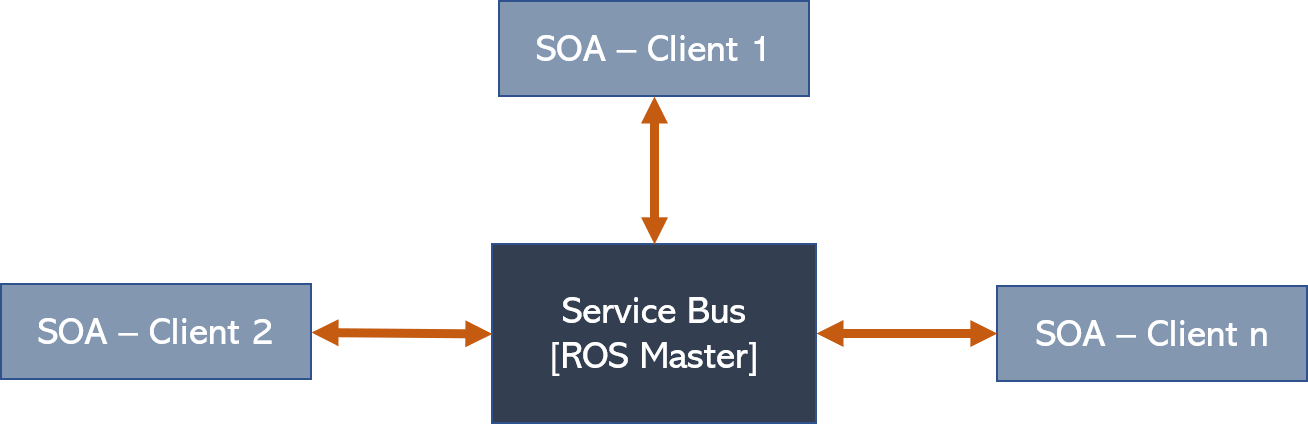
\includegraphics[scale=0.5]{"Grafiken/soa.png"}
	\caption{Service Oriented Architecture}
	\label{fig:meine-grafik}
\end{figure}
Bei der SOA spielt der (Enterprise) Service Bus eine zentrale Rolle. Er ist das Bindeglied zwischen allen anderen Knotenpunkten im Netzwerk und stellt sicher, dass die Kommunikation funktioniert. Bei ROS ist das der ROS-Master, der über den Befehl \code{roscore} gestartet werden kann. Über ihn kommunizieren die Knoten miteinander, wobei jeder Knoten eine logisch abgeschlossene Aufgabe übernimmt und von außen über eine API angesprochen werden kann. Im Fall des Quadrokopters existiert nun beispielsweise ein Knoten, der das Kamerabild publiziert, einer, der das Bild verarbeitet und einer, der die Steuerung auf Basis der Bilddaten durchführt. Durch diese Modularität gibt es einige Vorteile. So ist es damit sehr leicht einen Knoten auszutauschen, zu erweitern oder neue Knoten hinzuzufügen. Zudem ist das System deutlich stabiler als eine monolithische Lösung, da bei einem fehlerhaften Knoten nur die Knoten ausfallen, die von diesem Ausfall logisch betroffen sind. Alle unabhängigen Knoten werden weiterhin funktionieren. Bei einer monolithischen Lösung führt ein Modulausfall zum Ausfall des Gesamtsystems. 
\paragraph{}
Aber einer gewissen Granularität spricht man von Microservices. Diese folgen der Strategie 
"Erledige nur eine Aufgabe und erledige sie gut" %ToDo:\cite{riedel:it-arch}
Bei "normalen" SOAs sind die Knoten tendenziell groß und implementieren viele Funktionalitäten auf einmal. Microservices hingegen sind sehr klein und erledigen nur eine bestimmte Aufgabe. In der finalen Gesamtarchitektur kommen Knoten zum Einsatz, die sowohl den normalen SOAs als auch den Microservices zugewiesen werden können.



\pagebreak
\subsection{Finale Gesamtarchitektur}
\begin{figure}[h]
	\centering
	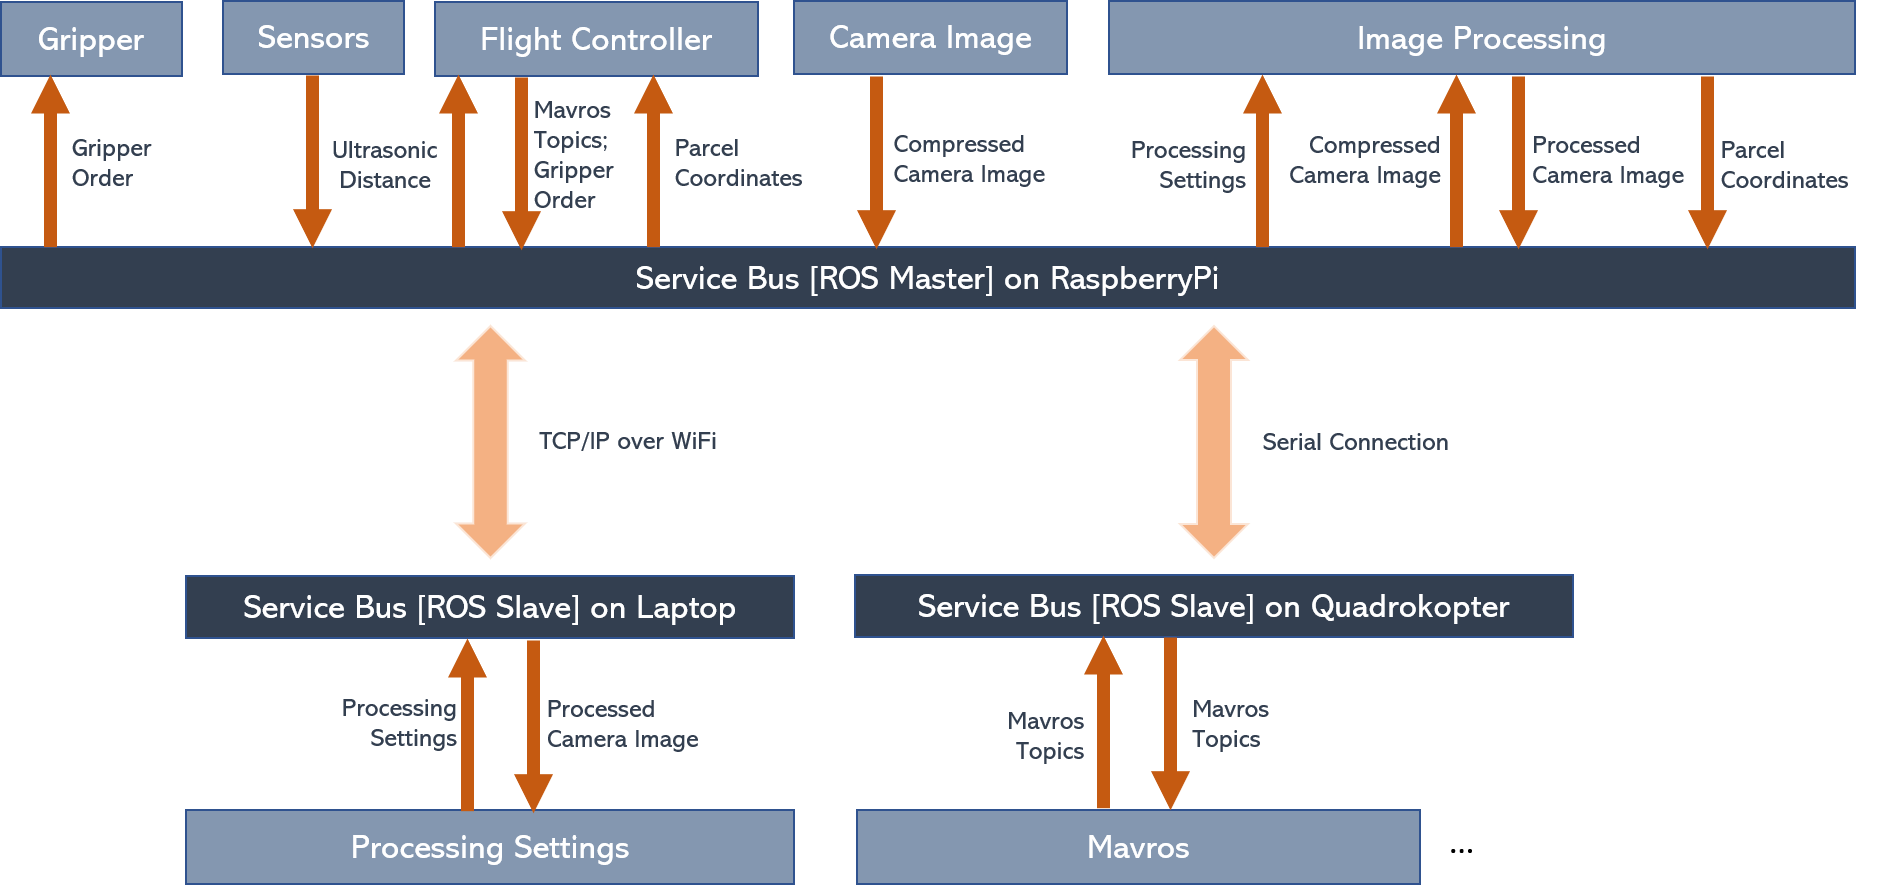
\includegraphics[scale=0.51]{"Grafiken/gesamtarchitektur.png"}
	\caption{Service Oriented Architecture}
	\label{fig:meine-grafik}
\end{figure}
In der finalen Gesamtarchitektur gibt es insgesamt drei ROS Instanzen: Die erste läuft auf dem Quadrokopter selber und dient als Schnittstelle zur Firmware des Quadrokopters. Der dazugehörige Knoten heißt Mavros, welcher mit MAVLink (Micro Air Vehicle Link) kommuniziert, das die gesamte tatsächliche Steuerung des Quadrokopters übernimmt. Dabei hat der ROS-Core jedoch keine Master-Funktion, sondern verbindet sich über eine serielle Schnittstelle mit dem ROS-Core auf dem RaspberryPi, auf dem der tatsächliche Master-ROS-Core läuft. Dieser ist in einem WLAN-Netzwerk mit einem Laptop, der für Debugging-Zwecke und zum Konfigurieren und Kontrollieren der Bildverarbeitung benötigt wird. Auch auf dem Laptop läuft ein ROS-Core, wobei auch dieser sich mit dem Master auf dem Raspberry Pi verbindet. Im folgenden werden nun die einzelnen Knoten genauer betrachtet.
\paragraph{Camera Image} ist ein einfacher Publisher, der das Bild der Dronenkamera komprimiert und über den Service Bus den anderen Knoten im Netzwerk zu Verfügung stellt.
\paragraph{Image Processing} empfängt die Bilddaten von Camera Image und wir zudem über das Topic Processing-Settings vom Laptop aus konfiguriert. Dieser Knoten filtert dann das Bild um anschließend die Position des Pakets zu ermitteln. Das gefilterte Bild und die Koordinaten des Pakets werden publiziert. 
\paragraph{Sensors} ist ein Knoten, der Sensordaten wie den Ultraschallsensor zum Boden aufbereitet, validiert und dann publiziert.
\paragraph{Flight Controller} ist die zentrale Steuereinheit der neuen Funktionalität. Er empfängt alle aufbereiteten Sensordaten wie die Koordinaten des Pakets, Ultraschalldistanz, Sensordaten der Drone etc. und führt die Suche und Anflug des Pakets durch. Er gibt die Flugsteuerbefehle an Mavros über die serielle Schnittstelle weiter und gibt Greifbefehle weiter.


\subsection{Softwareentwicklungsprozess}
Für eine effektive und effiziente Entwicklung des Softwaresystems ist die Nutzung geeigneter unterstützender Software unabdingbar. Daher soll nun die verwendete Toolchain kurz vorgestellt werden.
\subsubsection{ROS auf Ubuntu}
\paragraph{Setup} Sowohl die Entwicklung als auch die Runtime läuft auf Ubuntu 18.04. Das gilt also sowohl für Entwicklungsrechner, als auch für den Raspberry Pi, wobei bei diesem Ubuntu Mate eingesetzt wird. Der Vorteil ist, dass ROS nativ darauf funktioniert und sehr viele Bibliotheken für ROS bereits vorkompiliert zur Verfügung stehen. Es ist dabei für die aktuelle ROS-Version "Melodic" dringend davon abzuraten, das System auf einer Raspian-Installation laufen zu lassen, da man einerseits alle Pakete selber kompilieren muss und darüber hinaus viele der Abhängigkeiten von MAVROS nicht zu Verfügung stehen. Wichtig ist auch, dass "Melodic" ausschließlich von der Ubuntu-Version 18.04 unterstützt wird. Die Installation von ROS lässt sich auf Ubuntu nach Hinzufügen des Repositories über \code{sudo apt install ros-melodic-ros-base} einfach durchführen. Hierbei ist es empfehlenswert für den Raspberry Pi die \code{ros-base} Version und für den Entwicklungsrechner die \code{desktop-full} Version zu nehmen, da diese bereits die wichtigsten grafischen Werkzeuge installiert hat. Nachdem man nun noch rosdep initialisiert, welches das Arbeiten mit Softwareabhängigkeiten deutlich vereinfacht, müssen nun die mitinstallierten ROS-Pakete im aktuell genutzten Terminal mit Hilfe des \code{source} Befehls geladen werden. Bei einer Standardinstallation geht das mit \code{source /opt/ros/melodic/setup.bash}. 
\paragraph{Workspaces}
Alle eigenen Entwicklungen finden im sogenannten catkin-Workspace statt, worin sich die eigenen Pakete befinden. Dieser kann im home-Verzeichnis des Benutzers nach Erstellen des Verzeichnisses "catkin\_ws" mit \code{catkin\_make -DPYTHON\_EXECUTABLE=/usr/bin/python3} erstellt werden. Dabei muss \code{catkin\_make} jedes mal ausgeführt werden, wenn ein neues Paket erstellt wurde. Das kann mit dem Befehl \code{catkin\_create\_pkg my-package-name std\_msgs rospy roscpp} erreicht werden. Dadurch wir ein gleichnamiger Ordner im "src" Ordner des Workspaces erstellt, in dem die Sourcedateien abgelegt werden können. Um die neuen Pakete nun auch in ROS zu Verfügung zu haben, müssen diese auch im Terminal geladen werden. Das geht analog zum Laden der vorinstallierten Pakete mit \code{source \~/catkin\_ws/devel/setup.bash}. 
\paragraph{.bashrc}
Um nicht bei jedem neuen Terminal erst die Pakete manuell laden zu müssen, bietet Ubuntu die Möglichkeit dies automatisch zu tun. Dafür ist die Datei .bashrc zuständig, die sich im home-Verzeichnis eines jeden Benutzer befindet. In diese können die beiden Befehle einfach angehängt werden. Auch die Konfiguration für Gazebo (siehe Kapitel x.x.x) kann hier bereits erfolgen. Es sei aber zu erwähnen, dass dies nur so lange sinnvoll ist, wie ROS hauptsächlich auf dem System genutzt wird. 
\subsection{Entwicklungsumgebung und Versionsverwaltung}
Eine (integrierte) Entwicklungsumgebung sollte den Entwickler in seiner Arbeit unterstützen und ihm sich wiederholende oder logisch einfache, aber zeitaufwändige Schritte abnehmen. Für diese Entwicklung fiel daher die Wahl auf "PyCharm" der Firma JetBrains. Dieses bietet neben dem obligatorischen Texteditor mit integriertem Auto-Complete und Compiler Vorschläge zu Codeverbesserung Refactoring etc. Es macht hier jedoch Sinn sich eine der ROS-Erweiterungen für PyCharm zu installieren, damit die ROS-eigenen Python Bibliotheken auch korrekt erkannt werden. PyCharm arbeitet zudem mit Virtual Environments (venv), also einer abgekapselten, meist projektspezifischen Python-Installation, die nur die zusätzlichen Bibliotheken enthält, die für das aktuelle Projekt benötigt werden. Diese sollte bei allen Entwicklern identisch sein, um Versionsinkompatibilitäten zu vermeiden. Ein weitere Funktion von PyCharm ist die integrierte Versionsverwaltung, kurz VCS (Version Control System). Diese bietet eine direkte Anbindung an Git, das Versionen des Sourcecodes verwaltet und Teilentwicklungen in den verschieden Entwicklungszweigen (branch) der Entwickler effektiv zum Hauptzweig (master) zusammenbringt (merge). Konflikte, wenn beispielsweise eine Datei von zwei zu vereinenden Zweigen bearbeitet wurden, müssen jedoch oft von Hand gelöst werden. Deshalb macht es Sinn Funktionalitäten weitestgehend in einzelne Dateien zu unterteilen. \cite{martinez2013learning}

\subsection{Implementierung der Kommunikation in ROS}
\paragraph{}
Wie bereits erwähnt basiert ROS auf dem Publisher/Subscriber Prinzip. Ein Knoten kann in ROS sowohl Publisher als auch Subscriber sein und das auch für mehrere Topics. Die Topics sind dabei hierarchisch aufgebaut und gehen vom Groben ins Feine. So publiziert beispielsweise der "Camera Image" Knoten das komprimierte Bild in \code{/camera/image/compressed}. Anhand dieses Beispiels soll nun dargelegt werden, wie man prinzipiell bei der Erstellung eines Nodes vorgeht.
\subsubsection{Kamera Publisher}
Zunächst muss eine Datei mit dem Namen des Knotens und der Endung ".py" im entsprechenden Paketordner im src-Ordner des Catkin-Workspaces erstellt werden. Diese kann dann in PyCharm geöffnet werden, wenn nicht schon das gesamte Paket als Projekt geöffnet wurde.
Um klarzumachen, dass es sich hierbei um ein Python File handelt, muss die Datei mit \code{\#!/usr/bin/env python3} starten, um die Pythonumgebung auszuwählen. Es folgt nun für gewöhnlich die Lizenzerklärung zur Datei. Es sollten nun \code{numpy as np, time, sys, cv2, roslib, rospy} importiert werden, sowie \code{CompressedImage} aus der ROS-Bibliothek \code{sensor\_msgs.msg}. Es empfiehlt sich nun die gesamte Funktionalität mittels \code{def function\_name} in eine Funktion zu packen. Dort muss dann zunächst mit \code{pub = rospy.Publisher("", DataType)} ein Objekt erstellt werden, wobei hier das Topic \code{"/camera/image/compressed"}, sowie der Datentyp \code{CompressedImage} dem Konstruktor übergeben werden müssen. Mit \code{rospy.init\_node('node\_name', anonymous=True)} registriert sich der Knoten nun am ROS-Service-Bus. Nun wird die Computerbildverarbeitungsbibliothek OpenCV genutzt, um mit \code{cap = cv2.VideoCapture(0)} ein Objekt zu erstellen, dass auf den Datenstrom der ersten angeschlossenen Kamera zugreift. Der nun folgende Code soll so lange ausgeführt werden, wie ROS aktiv ist. Dies lässt sich mit \code{while not rospy.is\_shutdown():} implementieren. Mit \code{ret, frame = cap.read()} wird nun der Datenstrom der Kamera ausgelesen und das aktuelle Bild in die Variable \code{frame} geschrieben. Jetzt muss mit \code{msg = CompressedImage()} ein Nachrichtenpaket des Typs \code{CompressedImage} erstellt werden, das mit \code{msg.header.stamp = rospy.Time.now()} um einen Zeitstempel erweitert wird und mit \code{msg.format = "jpeg"} das richtige Dateiformat erhält. Die Daten des Pakets werden mit der Property \code{msg.data} gesetzt. Diese müssen nun aus dem vorher gelesenen \code{frame} erstellt werden. Dafür wird zunächst mit \code{cv2.imencode('.jpg', frame)[1]} das \code{frame} mithilfe von OpenCV in ein JPEG umgewandelt und wird dann mit \code{np.array()} zu einem Bildarray transformiert wird und mit \code{tostring()} serialisiert wird. Nun ist Paket bereit mit \code{pub.publish(msg)} an den Service Bus gesendet zu werden. Die Funktion sollte nun mit \code{if \_\_name\_\_ == '\_\_main\_\_': function\_name()} aufgerufen werden, wobei es Sinn macht den Funktionsaufruf mit einer Ausnahmeregelung für die \code{rospy.ROSInterruptException} zu erweitern. 
\subsubsection{Kamera Subscriber}
Der dazugehörige Subscriber ist im Knoten "Image Processing" implementiert und ist dem Publisher gegenüber recht ähnlich aufgebaut. Hier wird jedoch ein Subscriber-Objekt mit \code{rospy.Subscriber("topic", DataType, callback)} erstellt, wobei callback die Callback-Funktion ist, die aufgerufen wird, wenn eine neue Nachricht in der Topic ankommt. In den Argumenten dieser Funktion eine Variable \code{msg} definiert sein, in der die Nachricht bei Empfang gespeichert wird. Der Inhalt der Nachricht kann mit \code{msg.data} aufgerufen werden und mit \code{np.fromstring(data, np.uint8)} zuerst zu einem \code{numpy}-Array deserialisiert und dann mit \code{cv2.imdecode(np\_arr, cv2.IMREAD\_COLOR)} zu einem für OpenCV verarbeitbarem Format dekodiert werden. Der darauf folgende Code zur Bildverarbeitung ist in Kapitel x.x.x. beschrieben. \cite{aniskoubaa2019}
\subsection{Starten und Automation eines ROS-Systems}
Damit die Knoten auch lauffähig sind, müssen die Dateien zunächst mit \code{chmod +x} für den Kernel ausführbar gekennzeichnet werden. Nun können, nachdem \code{roscore} ausgeführt wurde, in einem jeweils neuen Terminaltab mit \code{rosrun paketname knotenname.py} die verschiedenen Knoten ausgeführt werden. Mit \code{rostopic echo /topic/name} können die Nachrichten der verschiedenen Topics überwacht werden. Um das alle nicht jedes Mal von Hand machen zu müssen, gibt es bei ROS sogenannte Launch-Files, die, wenn ausgeführt, nicht nur einen ROS-Core ausführen, sondern auch alle notwendigen Knoten startet, Umgebungsvariablen setzt etc. Das Launch File basiert auf XML und enthält innerhalb des \code{<launch></launch>} Tags alle Komponenten. Ein Knoten ist dabei recht selbsterklärend aufgebaut: \code{<node name="CameraImagePub" pkg="parcelcopter" type="CameraImagePub.py" />}. Innerhalb des Tags können außerdem Startparameter mit \code{arg} definiert werden.Mit dem \code{env}-Tag können zudem Umgebungsvariablen gesetzt werden. 

\paragraph{}Man bemerke hier die Modularität und Stabilität von ROS. Denn die Knoten geben keinen Fehler aus, obwohl ein anderer Knoten, der eigentlich für die Ausführung von Nöten ist, noch gar nicht gestartet ist. Sobald dieser bereit ist, fangen die davon abhängigen Knoten automatisch an zu arbeiten. 

\subsection{Mavros und Simulation}
\subsection{Dronensteuerung}
